\sect{Vektoren}

\ssect{Definition}

Ein Vektor ist ein Object mit \textbf{Betrag} und \textbf{Richtung} hat.

\ssect{Operationen}

\sssect{Addition}

\begin{multicols}{2}
    \[\vec{a} + \vec{b} = \left(
    \begin{array}{c}
        a_x + b_x \\
        a_y + b_y
    \end{array}
    \right)\]
    \begin{center}
        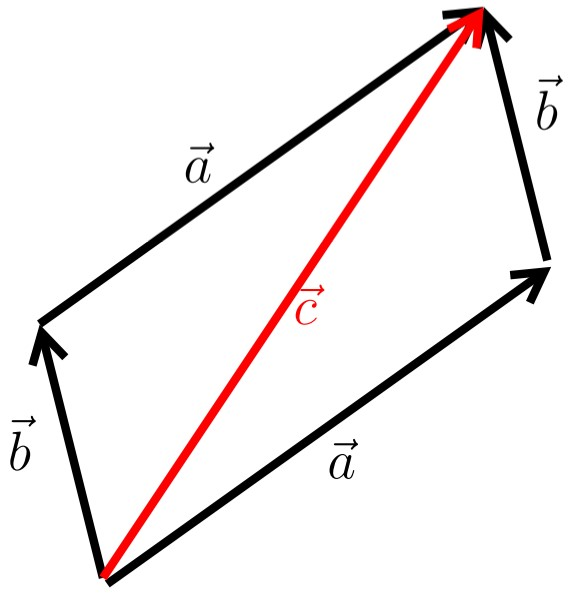
\includegraphics[scale=0.133]{vektor-addition}
    \end{center}
\end{multicols}

\textbf{Rechenregeln:}
\begin{enumerate}
    \item \textbf{Kommutativgesetz:} $\vec{a} + \vec{b} = \vec{b} + \vec{a}$
    \item \textbf{Assoziativgesetz:} $(\vec{a} + \vec{b}) + \vec{c} = \vec{a} + (\vec{b} + \vec{c})$
    \item Der Nullvektor ist das \textbf{Neutralelement}: $\vec{a} + \vec{0} = \vec{a}$
    \item Zu jedem Vektor $\vec{a}$ gibt es genau einen \textbf{Gegenvektor} $-\vec{a} \in \R^n$ mit $\vec{a} + (-\vec{a}) = \vec{0}$
\end{enumerate}

\sssect{Skalare Multiplikation}

\vspace{0.5em}

\begin{multicols}{2}
    \[\lambda \cdot \vec{a} = \left(
    \begin{array}{c}
        \lambda \cdot \vec{a_x} \\
        \lambda \cdot \vec{a_y}
    \end{array}
    \right)\]

    $\vec{a}$ und $\vec{b}$ heissen \textbf{kollinear}, falls $\vec{a} = \lambda \vec{b}$.
    Andernfalls heissen sie \textbf{windschief}.
\end{multicols}

Seien $\vec{w}_1, \dots, \vec{w}_m$ Vektoren und $a_1, \dots, a_m$ reellen Zahlen mit $m \in \N$.
Der Vektor \[\vec{v} = a_1 \vec{w}_1 + \dots + a_m \vec{w}_m \coloneqq \sum_{i=1}^{m} a_i \vec{w}_i\] heisst eine \textbf{Linearkombination} von den Vektoren.
Die Zahlen $a_1, \dots, a_m$ heissen \textbf{Koeffizienten}.

\sssect{Betrag}

\vspace{0.5em}

\begin{multicols}{2}
    \begin{center}
        $|\vec{a}| = \sqrt{a_x^2 + a_y^2 + a_z^2}$
    \end{center}

    \textbf{Einheitsvektor}: $|\vec{e}| = 1$
\end{multicols}

\sssect{Skalarprodukt}

Das \textbf{Skalarprodukt} (Engl.\ dot product) berechnet sich aus:
\begin{itemize}
    \item $\vec{a} \cdot \vec{b} = |\vec{a}| |\vec{b}| \cos(\varphi)$
    \item $\vec{a} \cdot \vec{b} = |\vec{a}|^2$
    \item $\vec{a} \cdot \vec{b} = a_1 b_1 + \dots + a_n b_n = \sum_{i=1}^{n} a_i b_i$
\end{itemize}

\textbf{Anmerkung:}
\begin{itemize}
    \item Das Skalarprodukt wird auch als $(\vec{a}, \vec{b})$, $\langle \vec{a} | \vec{b} \rangle$ oder $\vec{a}^T \vec{b}$ geschrieben.
    \item Der Winkel $\varphi$ ist stets \textbf{der kleinere} der beiden Winkel zwischen den Vektoren: $0^{\circ} \leq \varphi \leq 180^{\circ}$
\end{itemize}

Zwei Vektoren sind \textbf{orthogonal} zueinander, falls: \[\vec{a} \cdot \vec{b} = 0 \Leftrightarrow \vec{a} \perp \vec{b}\]

Der Winkel zwischen zwei Vektoren berechnet sich aus: \[\varphi = \arccos \left( \frac{\vec{a} \cdot \vec{b}}{|\vec{a}| |\vec{b}|} \right)\]

\sssect{Vektorprodukt}

\begin{itemize}
    \item $|\vec{a} \times \vec{b}| = |\vec{a}| \cdot |\vec{b}| \sin(\varphi)$
    \item $\vec{a} \times \vec{b}$ \textbf{ist orthogonal zu $\vec{a}$ und $\vec{b}$}
    \item $\vec{a} \times \vec{b} \neq \vec{b} \times \vec{a}$
\end{itemize}
\[\vec{a} \times \vec{b} = \left(
\begin{array}{c}
    a_x \\ a_y \\ a_z
\end{array}
\right) \times \left(
\begin{array}{c}
    b_x \\ b_y \\ b_z
\end{array}
\right) = \left(
\begin{array}{c}
    a_y b_z - a_z b_y \\
    a_z b_x - a_x b_z \\
    a_x b_y - a_y b_x
\end{array}
\right)\]
\textbf{Anmerkung:}
\begin{itemize}
    \item Das Vektorprodukt ist im Gegensatz zum Skalarprodukt eine \textbf{vektorielle Grösse} und wird auch als \textbf{äusseres Produkt} oder \textbf{Kreuzprodukt} bezeichnet.
    \item Das Vektorprodukt existiert im Gegensatz zum Skalarprodukt \textbf{nur} für dreidimensionale Vektoren.
    \item Der Betrag des Vektorproduktes entspricht dem \textbf{Flächeninhalt} des von den Vektoren $\vec{a}$ und $\vec{b}$ aufgespannten Parallelogramms.
    \item $\vec{a} \times \vec{b} = 0 \Leftrightarrow$ $\vec{a}$ und $\vec{b}$ sind \textbf{kollinear}
    \item $\vec{a} \times \vec{b} = -(\vec{b} \times \vec{a})$
\end{itemize}
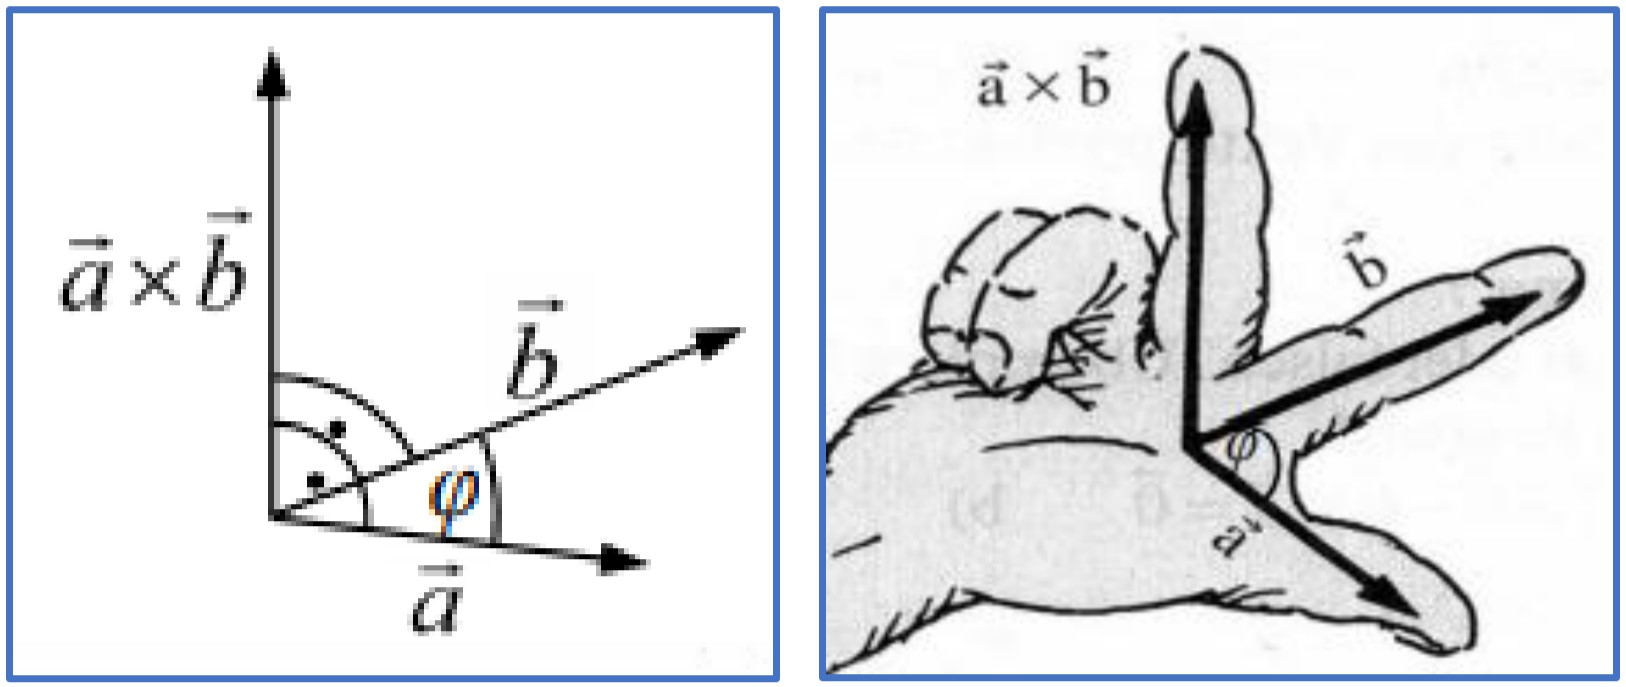
\includegraphics[scale=0.21]{vektorprodukt}

\sssect{Komplanar}

$\vec{a}$, $\vec{b}$ und $\vec{c}$ heissen \textbf{komplanar}, wenn sie auf gleichen Ebene liegen.
$\vec{a}$ lässt sich dann als Linearkombination von $\vec{b}$ und $\vec{c}$ ausdrücken:
\[\vec{a} = \lambda \vec{b} + \mu \vec{c}\]

\begin{center}
    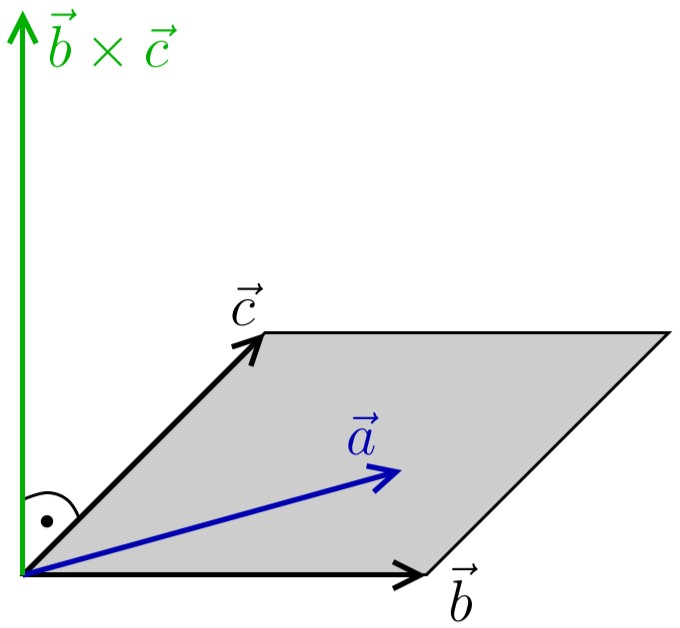
\includegraphics[scale=0.18]{komplanar}
\end{center}

\ssect{Geraden}

\sssect{Parametergleichung}

\vspace{0.5em}
\begin{multicols}{2}
    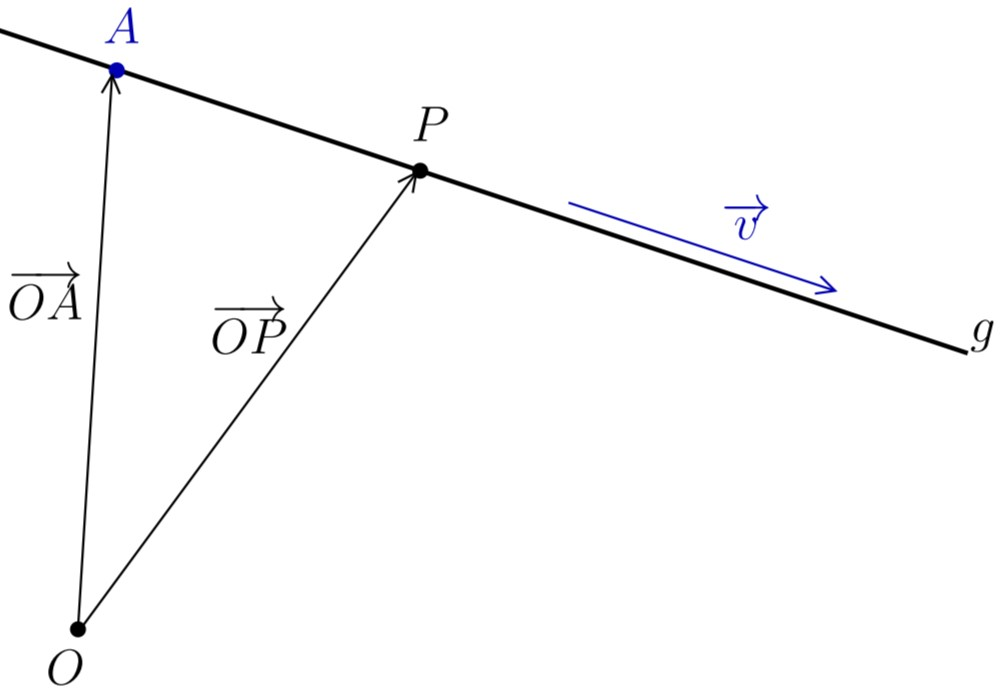
\includegraphics[scale=0.15]{parametergleichung-gerade}

    $g$ sei eine Gerade, die durch den Punkt $A$ und parallel zum Richtungsvektor $\vec{v}$ verläuft.
    Eine \textbf{Parameterdarstellung} dieser Geraden lautet:
    $g: \vec{OA} + \lambda \vec{v}$
\end{multicols}

Der Punkt $A$ heisst \textbf{Aufpunkt}, der Vektor $\vec{OA}$ heisst \textbf{Stützvektor} und der Vektor $\vec{v}$ heisst \textbf{Richtungsvektor}.

Ein Punkt $P$ liegt genau dann auf $g$, wenn es ein $\lambda$ gibt, sodass gilt:
$\vec{OP} = \vec{OA} + \lambda \vec{v}$

\sssect{Koordinatengleichung}

\begin{center}
    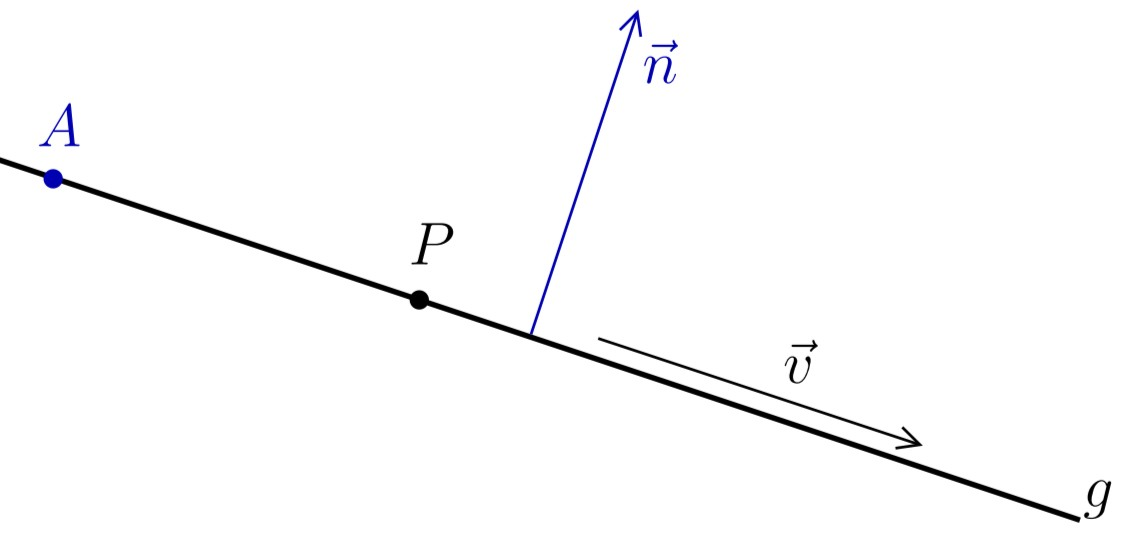
\includegraphics[scale=0.17]{koordinatengleichung-gerade}
\end{center}

$g$ sei eine Gerade, die durch den Punkt $A = (a_x, a_y)$ und senkrecht zum Normalenvektor $n = (a \ b)^T$ verläuft.
Die \textbf{Koordinatengleichung} lautet:
\[\vec{n} \cdot \vec{OP} - n \cdot \vec{OA} = 0\]
Oder in der Komponentenschreibweise:
\[ax + by + c = 0\]
wobei $c = -\vec{n} \cdot \vec{OA} = -(a a_x + b a_y)$ und $P = (x, y)$.

\textbf{Beispiel:} $A = (4 \ 6)^T$ und $\vec{n} = (3 \ -1)^T$
\[g: 3x - y - (3 \cdot 4 - 1 \cdot 6) = 0 \Leftrightarrow 3x - y - 6 = 0\]


\sssect{Gegenseitige Lage in der Ebene}

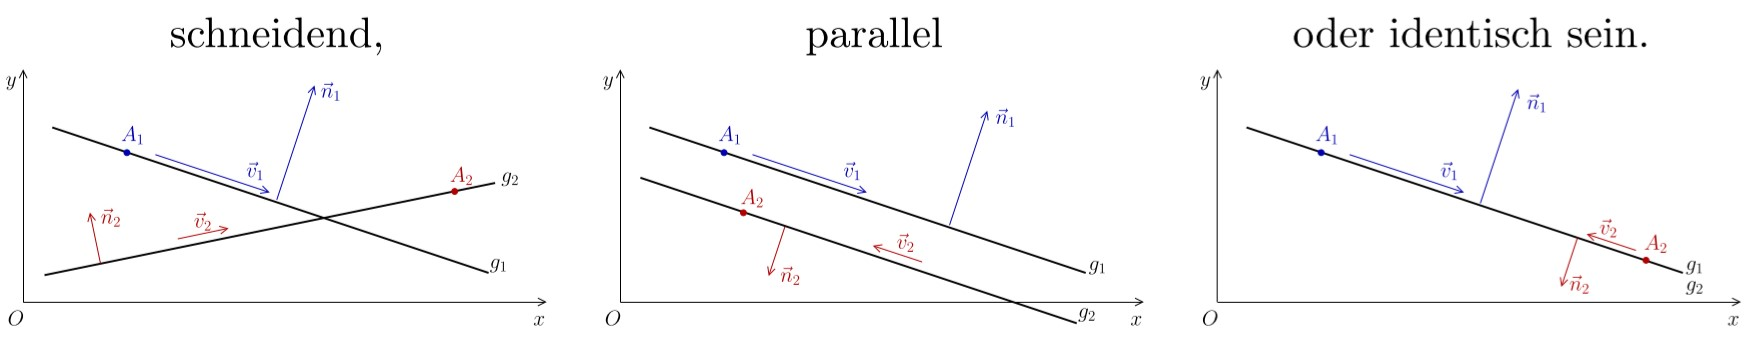
\includegraphics[scale=0.2]{gegenseitige-lage-geraden-ebene}

\sssect{Gegenseitige Lage im Raum}

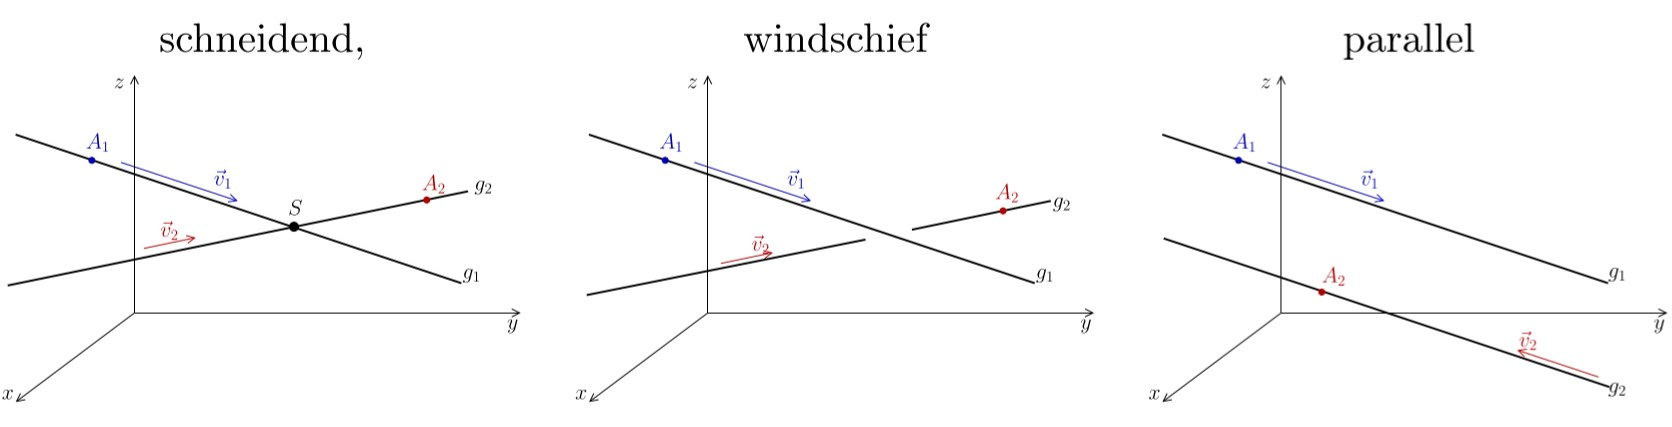
\includegraphics[scale=0.21]{gegenseitige-lage-geraden-raum}

\ssect{Ebenen}

\sssect{Parametergleichung}

\vspace{0.5em}
\begin{multicols}{2}
    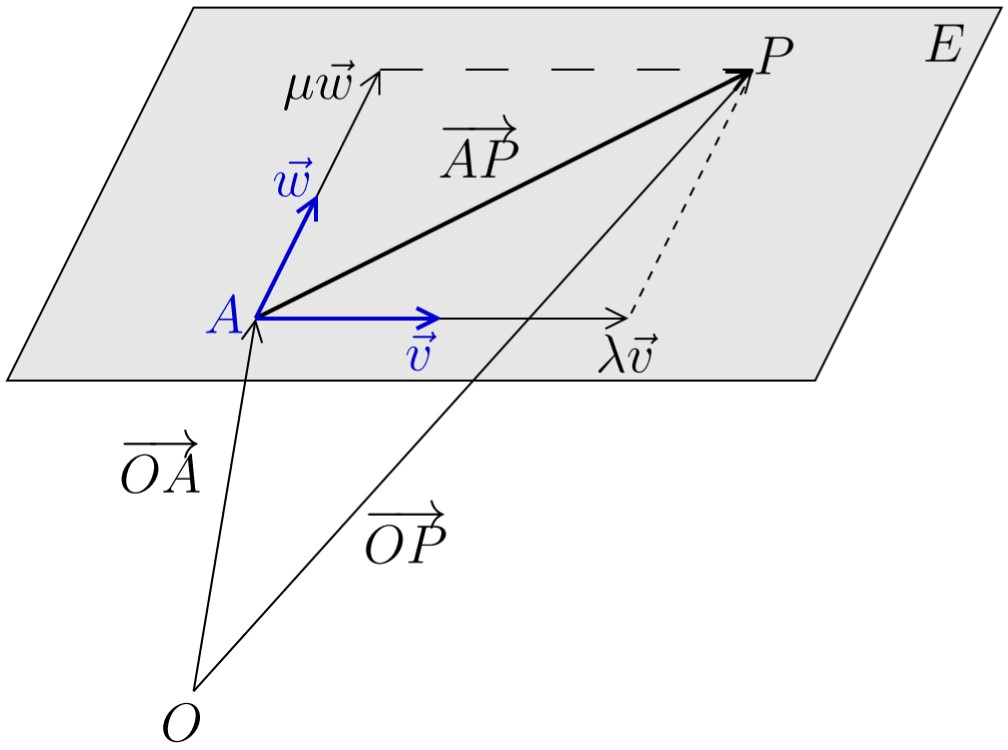
\includegraphics[scale=0.17]{parametergleichung-ebene}

    $E$ sei eine Ebene, die durch den Punkt $A$ und parallel zu zwei nichtkollinearen Vektoren $\vec{v}$ und $\vec{w}$ verläuft.
    Die \textbf{vektorielle Parameterform} der Ebene-Gleichung lautet:
    \[\vec{OP} = \vec{OA} + \lambda \vec{v} + \mu \vec{w}\]
\end{multicols}

$\vec{v}$ und $\vec{w}$ heissen \textbf{Richtungsvektoren} der Ebene $E$.

\sssect{Koordinatengleichung}

Ein auf der Ebene $E$ senkrecht stehender Vektor $\vec{n}$ heisst \textbf{Normalenvektor der Ebene}: $\vec{n} = \vec{v} \times \vec{w}$

\vspace{0.5em}
\begin{multicols}{2}
    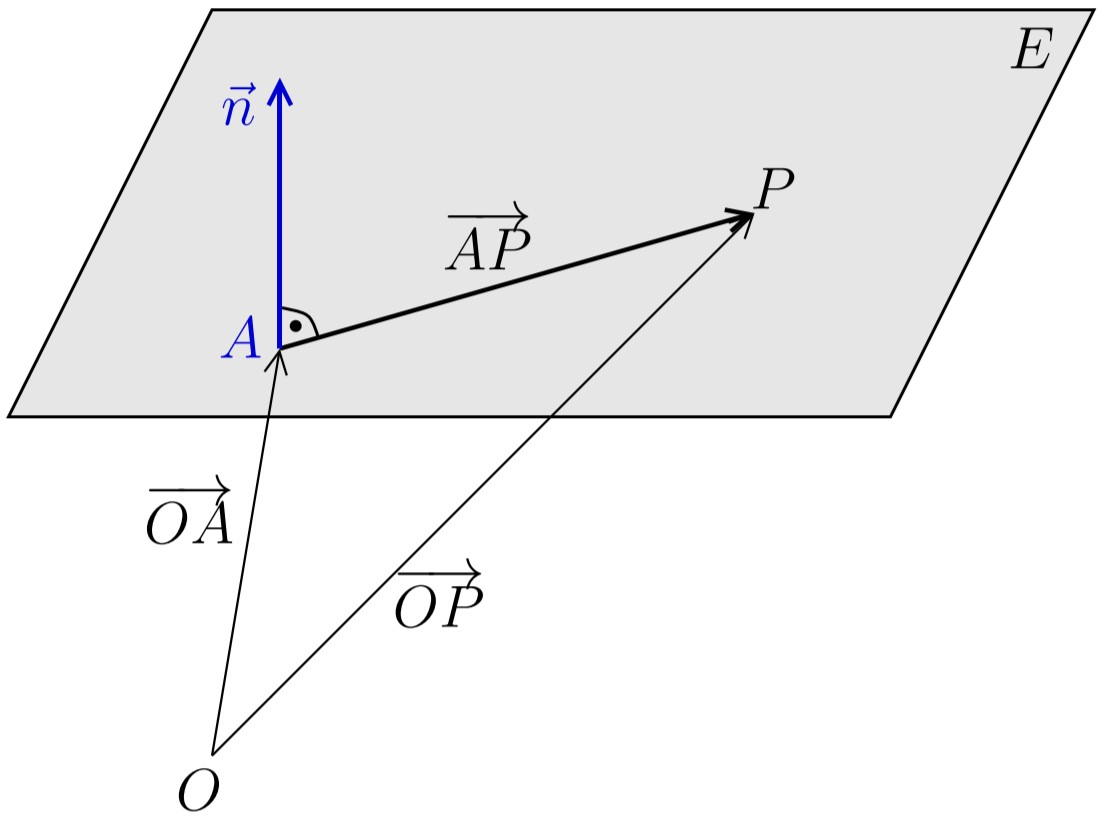
\includegraphics[scale=0.15]{koordinatengleichung-ebene}

    $E$ sei eine Ebene, die durch den Punkt $A = (a_x, a_y, a_z)$ und senkrecht zum Normalenvektor $n = (a \ b \ c)^T$ verläuft.
    Die \textbf{Koordinatengleichung} lautet:
    \[E: \vec{n} \cdot (\vec{OP} - \vec{OA}) = 0\]
\end{multicols}

Oder in der Komponentenschreibweise:
\[E: ax + by + cz + d = 0\]
wobei $d = -\vec{n} \cdot \vec{OA} = -(a a_x + b a_y + c a_z)$ und $P = (x, y, z)$.

\textbf{Beispiel:} $A = (2 \ -5 \ 3)^T$ und $\vec{n} = (4 \ 2 \ 5)$
\[4x + 2y + 5z - (4 \cdot 2 + 2 \cdot (-5) + 5 \cdot 3) = 0 \Leftrightarrow 4x + 2y + 5z - 13 = 0\]
Der Punkt $Q(0; 4; 1)$ gehört zur Ebene, da
\[4 \cdot 0 + 2 \cdot 4 + 5 \cdot 1 - 13 = 8 + 5 - 13 = 0\]

\sssect{Gegenseitige Lage im Raum}

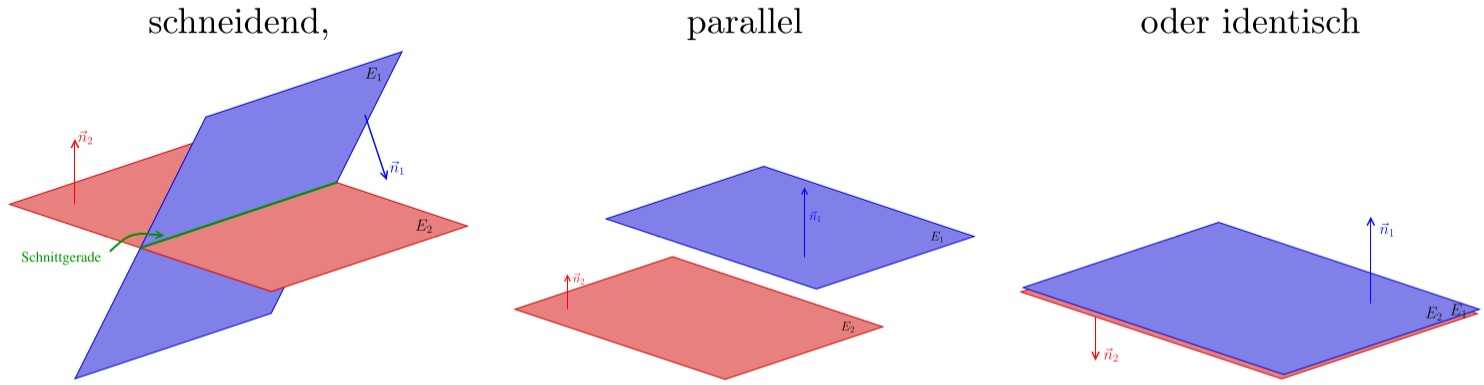
\includegraphics[scale=0.23]{gegenseitige-lage-ebenen-raum}

\ssect{Abständen}

\sssect{Abstand Punkt-Gerade in der Ebene}

\begin{center}
    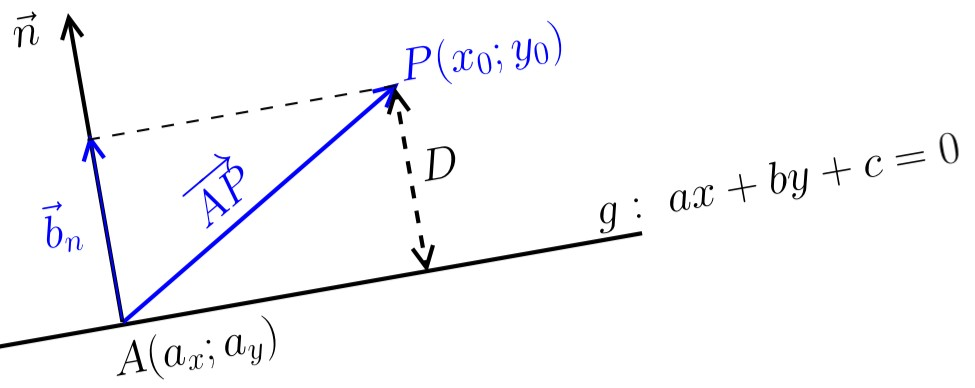
\includegraphics[scale=0.22]{abstand-punkt-gerade-ebene}
\end{center}

Der Abstand $D$ eines beliebigen Punktes $P(x_0, y_0)$ von der Geraden $g: ax + by + c = 0$ berechnet sich aus:
\[D = \frac{|\vec{AP} \cdot \vec{n}|}{|\vec{n}|} = \frac{|a x_0 + b y_0 + c|}{\sqrt{a^2 + b^2}}\]

\textbf{Beispiel:} Abstand des Punktes $P(5;7)$ von der Gerade $g: 3x + 4y + 15 = 0$:
\[D = \frac{|3 \cdot 5 + 4 \cdot (-7) + 15|}{\sqrt{3^2 + 4^2}} = \frac{|15 - 28 + 15|}{\sqrt{25}} = \frac{2}{5}\]

\sssect{Abstand Punkt-Gerade im Raum}

\begin{center}
    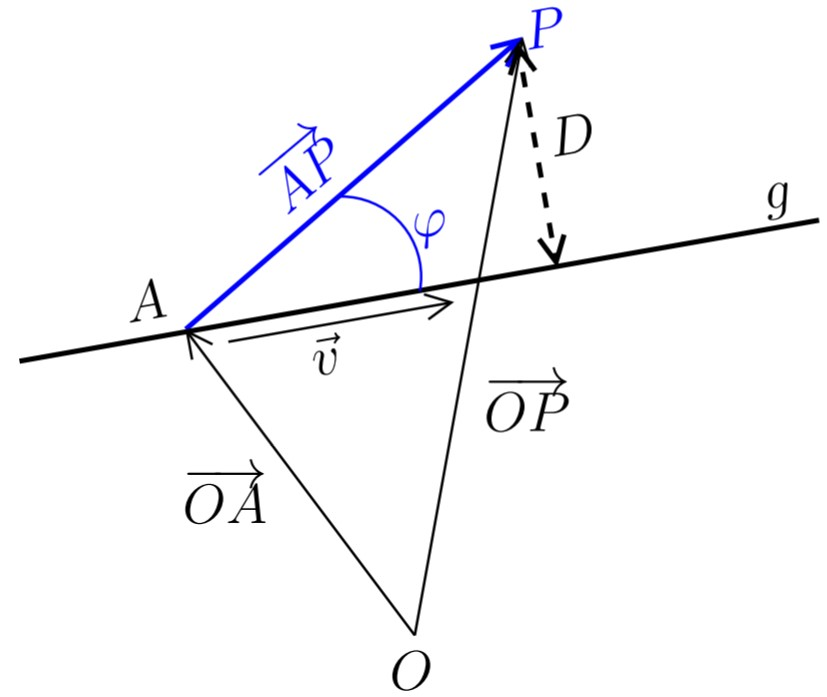
\includegraphics[scale=0.18]{abstand-punkt-gerade-raum}
\end{center}

Der Abstand $D$ eines beliebigen Punktes $P$ von der Geraden $g: \vec{OA} + \lambda \vec{v}$ berechnet sich aus:
\[D = \frac{|\vec{v} \times \vec{AP}|}{|\vec{v}|}\]

\textbf{Beispiel:}
Die Parametergleichung einer Geraden $g$ lautet:
\[g: \vec{OA} + \lambda \vec{v} = \left(
\begin{array}{c}
    1 \\ 0 \\ 1
\end{array}
\right) + \lambda \left(
\begin{array}{c}
    2 \\ 5 \\ 2
\end{array}
\right)\]
Wir berechnen den Abstand $D$ von $P(5;3;-2)$ zu $g$.
Zuerst berechnen wir das Vektorprodukt $\vec{v} \times \vec{AP}$:
\[\vec{v} \times \vec{AP} = \left(
\begin{array}{c}
    2 \\ 5 \\ 2
\end{array}
\right) \times \left(
\begin{array}{c}
    5 - 1 \\
    3 - 0 \\
    -2 - 1
\end{array}
\right) = \left(
\begin{array}{c}
    2 \\ 5 \\ 2
\end{array}
\right) \times \left(
\begin{array}{c}
    4 \\ 3 \\ -3
\end{array}
\right) = \left(
\begin{array}{c}
    -21 \\ 14 \\ -14
\end{array}
\right)\]
Daraus folgt:
\[|\vec{v} \times \vec{AP}| = \sqrt{(-21)^2 + 14^2 + (-14)^2} = \sqrt{833}\]
Wir müssen noch den Betrag von $\vec{v}$ berechnen:
\[|\vec{v}| = \sqrt{2^2 + 5^2 + 2^2} = \sqrt{33}\]
Somit: $D = \frac{|\vec{v} \times \vec{AP}|}{|\vec{v}|} = \frac{\sqrt{833}}{\sqrt{33}} \approx 5.02$

\sssect{Abstand Punkt-Ebene}

\begin{center}
    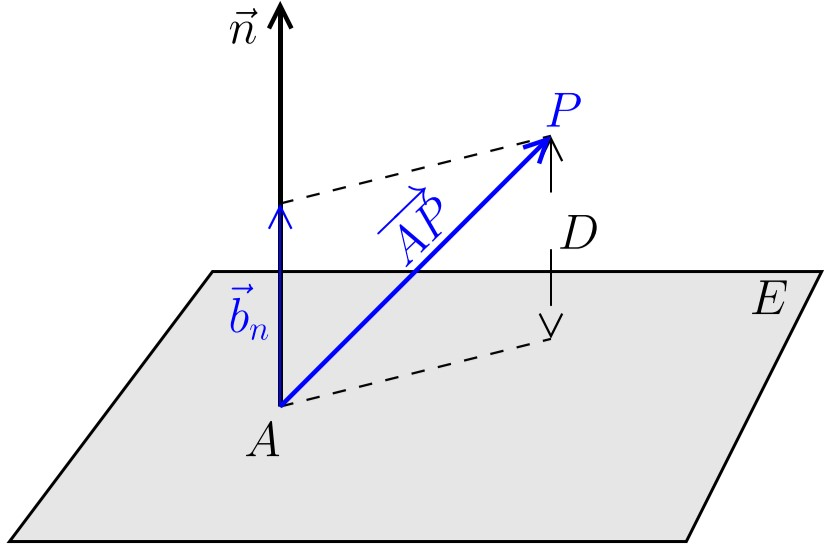
\includegraphics[scale=0.18]{abstand-punkt-ebene}
\end{center}

Der Abstand $D$ eines beliebigen Punktes $P(x_0, y_0, z_0)$ von der Ebene $E: ax + by + cz + d = 0$ berechnet sich aus:
\[D = \frac{|\vec{AP} \cdot \vec{n}|}{|\vec{n}|} = \frac{|a x_0 + b y_0 + c z_0 + d|}{\sqrt{a^2 + b^2 + c^2}}\]

\textbf{Beispiel:} Abstand von Punkt $P(1;0;-2)$ und der Ebene $E\colon -2x + y - 3z - 18 = 0$:
\[D = \frac{|-2 \cdot 1 + 1 \cdot 0 - 3 \cdot (-2) -18|}{\sqrt{(-2)^2 + 1^2 + (-3)^2}} = \frac{|-14|}{\sqrt{14}} = \frac{14}{\sqrt{14}} \approx 3.74\]